%%% The main file. It contains definitions of basic parameters and includes all other parts.

%% Settings for single-side (simplex) printing
% Margins: left 40mm, right 25mm, top and bottom 25mm
% (but beware, LaTeX adds 1in implicitly)
\documentclass[12pt,a4paper]{report}
\setlength\textwidth{145mm}
\setlength\textheight{247mm}
\setlength\oddsidemargin{15mm}
\setlength\evensidemargin{15mm}
\setlength\topmargin{0mm}
\setlength\headsep{0mm}
\setlength\headheight{0mm}
% \openright makes the following text appear on a right-hand page
\let\openright=\clearpage

%% Settings for two-sided (duplex) printing
% \documentclass[12pt,a4paper,twoside,openright]{report}
% \setlength\textwidth{145mm}
% \setlength\textheight{247mm}
% \setlength\oddsidemargin{14.2mm}
% \setlength\evensidemargin{0mm}
% \setlength\topmargin{0mm}
% \setlength\headsep{0mm}
% \setlength\headheight{0mm}
% \let\openright=\cleardoublepage

%% Generate PDF/A-2u
\usepackage[a-2u]{pdfx}

%% Character encoding: usually latin2, cp1250 or utf8:
\usepackage[utf8]{inputenc}

%% Prefer Latin Modern fonts
\usepackage{lmodern}

%% Further useful packages (included in most LaTeX distributions)
\usepackage{amsmath}        % extensions for typesetting of math
\usepackage{amsfonts}       % math fonts
\usepackage{amsthm}         % theorems, definitions, etc.
\usepackage{bbding}         % various symbols (squares, asterisks, scissors, ...)
\usepackage{bm}             % boldface symbols (\bm)
\usepackage{graphicx}       % embedding of pictures
\usepackage{fancyvrb}       % improved verbatim environment
\usepackage{natbib}         % citation style AUTHOR (YEAR), or AUTHOR [NUMBER]
\usepackage[nottoc]{tocbibind} % makes sure that bibliography and the lists
			    % of figures/tables are included in the table
			    % of contents
\usepackage{dcolumn}        % improved alignment of table columns
\usepackage{booktabs}       % improved horizontal lines in tables
\usepackage{paralist}       % improved enumerate and itemize
\usepackage{xcolor}         % typesetting in color
\usepackage{indentfirst}

%%% Basic information on the thesis
\setcounter{secnumdepth}{4}
\setcounter{tocdepth}{4}

% Thesis title in English (exactly as in the formal assignment)
\def\ThesisTitle{Automatic generation of medical reports from chest X-rays}

% Author of the thesis
\def\ThesisAuthor{Bc. Lukáš Chaloupský}

% Year when the thesis is submitted
\def\YearSubmitted{2022}

% Name of the department or institute, where the work was officially assigned
% (according to the Organizational Structure of MFF UK in English,
% or a full name of a department outside MFF)
\def\Department{Institute of Formal and Applied Linguistics}

% Is it a department (katedra), or an institute (ústav)?
\def\DeptType{Institute}

% Thesis supervisor: name, surname and titles
\def\Supervisor{Mgr. Rudolf Rosa, Ph.D.}

% Supervisor's department (again according to Organizational structure of MFF)
\def\SupervisorsDepartment{Institute of Formal and Applied Linguistics}

% Study programme and specialization
\def\StudyProgramme{Computer Science}
\def\StudyBranch{Software and Data Engineering}

% An optional dedication: you can thank whomever you wish (your supervisor,
% consultant, a person who lent the software, etc.)
\def\Dedication{%
First of all, I would like to thank my supervisor Mgr. Rudolf Rosa, Ph.D. for all his time, guidance and valuable advices he gave me while working on this thesis. I would also like to thank my parents for their unlimited support and patience during my studies.
}

% Abstract (recommended length around 80-200 words; this is not a copy of your thesis assignment!)
\def\Abstract{%
This thesis deals with the problem of automatic generation of medical reports in the Czech langugage based on the input chest X-ray images using deep neural networks. The first part deals with the analysis of problem itself including comparison of existing solutions from several common points of view. In order to interpret medical images in the Czech language we present a fine-tuned a Czech GPT2 model specialized on medical texts based on the original pre-trained English GPT2 model along with its evaluation. In the second part the created Czech GPT2 is used for training neural network model for generating medical reports. The training was conducted on freely available data along with data pre-processing and their adjustment for the Czech language. Furthermore the model results are discussed and evaluated using standard metrics for natural language processing to determine the performance.
}

% 3 to 5 keywords (recommended), each enclosed in curly braces
\def\Keywords{%
{natural language processing}, {image captioning}, {x-ray}, {medical report generation}
}

%% The hyperref package for clickable links in PDF and also for storing
%% metadata to PDF (including the table of contents).
%% Most settings are pre-set by the pdfx package.
\hypersetup{unicode}
\hypersetup{breaklinks=true}

% Definitions of macros (see description inside)
%%% This file contains definitions of various useful macros and environments %%%
%%% Please add more macros here instead of cluttering other files with them. %%%

%%% Minor tweaks of style

% These macros employ a little dirty trick to convince LaTeX to typeset
% chapter headings sanely, without lots of empty space above them.
% Feel free to ignore.
\makeatletter
\def\@makechapterhead#1{
  {\parindent \z@ \raggedright \normalfont
   \Huge\bfseries \thechapter. #1
   \par\nobreak
   \vskip 20\p@
}}
\def\@makeschapterhead#1{
  {\parindent \z@ \raggedright \normalfont
   \Huge\bfseries #1
   \par\nobreak
   \vskip 20\p@
}}
\makeatother

% This macro defines a chapter, which is not numbered, but is included
% in the table of contents.
\def\chapwithtoc#1{
\chapter*{#1}
\addcontentsline{toc}{chapter}{#1}
}

% Draw black "slugs" whenever a line overflows, so that we can spot it easily.
\overfullrule=1mm

%%% Macros for definitions, theorems, claims, examples, ... (requires amsthm package)

\theoremstyle{plain}
\newtheorem{thm}{Theorem}
\newtheorem{lemma}[thm]{Lemma}
\newtheorem{claim}[thm]{Claim}

\theoremstyle{plain}
\newtheorem{defn}{Definition}

\theoremstyle{remark}
\newtheorem*{cor}{Corollary}
\newtheorem*{rem}{Remark}
\newtheorem*{example}{Example}

%%% An environment for proofs

\newenvironment{myproof}{
  \par\medskip\noindent
  \textit{Proof}.
}{
\newline
\rightline{$\qedsymbol$}
}

%%% An environment for typesetting of program code and input/output
%%% of programs. (Requires the fancyvrb package -- fancy verbatim.)

\DefineVerbatimEnvironment{code}{Verbatim}{fontsize=\small, frame=single}

%%% The field of all real and natural numbers
\newcommand{\R}{\mathbb{R}}
\newcommand{\N}{\mathbb{N}}

%%% Useful operators for statistics and probability
\DeclareMathOperator{\pr}{\textsf{P}}
\DeclareMathOperator{\E}{\textsf{E}\,}
\DeclareMathOperator{\var}{\textrm{var}}
\DeclareMathOperator{\sd}{\textrm{sd}}

%%% Transposition of a vector/matrix
\newcommand{\T}[1]{#1^\top}

%%% Various math goodies
\newcommand{\goto}{\rightarrow}
\newcommand{\gotop}{\stackrel{P}{\longrightarrow}}
\newcommand{\maon}[1]{o(n^{#1})}
\newcommand{\abs}[1]{\left|{#1}\right|}
\newcommand{\dint}{\int_0^\tau\!\!\int_0^\tau}
\newcommand{\isqr}[1]{\frac{1}{\sqrt{#1}}}

%%% Various table goodies
\newcommand{\pulrad}[1]{\raisebox{1.5ex}[0pt]{#1}}
\newcommand{\mc}[1]{\multicolumn{1}{c}{#1}}


% Title page and various mandatory informational pages
\begin{document}
%%% Title page of the thesis and other mandatory pages

%%% Title page of the thesis

\pagestyle{empty}
\hypersetup{pageanchor=false}
\begin{center}

\centerline{\mbox{
\includegraphics[width=166mm]{../img/logo-en.pdf}}}

\vspace{-8mm}
\vfill

{\bf\Large MASTER THESIS}

\vfill

{\LARGE\ThesisAuthor}

\vspace{15mm}

{\LARGE\bfseries\ThesisTitle}

\vfill

\Department

\vfill

{
\centerline{\vbox{\halign{\hbox to 0.45\hsize{\hfil #}&\hskip 0.5em\parbox[t]{0.45\hsize}{\raggedright #}\cr
Supervisor of the master thesis:&\Supervisor \cr
\noalign{\vspace{2mm}}
Study programme:&\StudyProgramme \cr
\noalign{\vspace{2mm}}
Study branch:&\StudyBranch \cr
}}}}

\vfill

% Zde doplňte rok
Prague \YearSubmitted

\end{center}

\newpage

%%% Here should be a bound sheet included -- a signed copy of the "master
%%% thesis assignment". This assignment is NOT a part of the electronic
%%% version of the thesis. DO NOT SCAN.

%%% A page with a solemn declaration to the master thesis

\openright
\hypersetup{pageanchor=true}
\pagestyle{plain}
\pagenumbering{roman}
\vglue 0pt plus 1fill

\noindent
I declare that I carried out this master thesis independently, and only with the cited
sources, literature and other professional sources. It has not been used to obtain another
or the same degree.

\medskip\noindent
I understand that my work relates to the rights and obligations under the Act No.~121/2000 Sb.,
the Copyright Act, as amended, in particular the fact that the Charles
University has the right to conclude a license agreement on the use of this
work as a school work pursuant to Section 60 subsection 1 of the Copyright~Act.

\vspace{10mm}

\hbox{\hbox to 0.5\hsize{%
In \hbox to 6em{\dotfill} date \hbox to 6em{\dotfill}
\hss}\hbox to 0.5\hsize{\dotfill\quad}}
\smallskip
\hbox{\hbox to 0.5\hsize{}\hbox to 0.5\hsize{\hfil Author's signature\hfil}}

\vspace{20mm}
\newpage

%%% Dedication

\openright

\noindent
\Dedication

\newpage

%%% Mandatory information page of the thesis

\openright

\vbox to 0.5\vsize{
\setlength\parindent{0mm}
\setlength\parskip{5mm}

Title:
\ThesisTitle

Author:
\ThesisAuthor

\DeptType:
\Department

Supervisor:
\Supervisor, \SupervisorsDepartment

Abstract:
\Abstract

Keywords:
\Keywords

\vss}

\newpage

\openright
\pagestyle{plain}
\pagenumbering{arabic}
\setcounter{page}{1}


%%% A page with automatically generated table of contents of the master thesis

\tableofcontents

%%% Each chapter is kept in a separate file
\chapter*{Introduction}
\addcontentsline{toc}{chapter}{Introduction}

In hospital, inspecting the X-rays and writing corresponding medical reports is a hard work that requires experienced specialized doctors, of which there are not many. A great deal of people visit hospitals daily and X-rays are taken for many of them. Automatic interpretation of X-ray image has a great potential to improve health care and it could be particulary helpful to doctors in order to distinguish serious cases from the ordinary ones and overall accelerate and improve their work.\\

Automatic generation of radiology reports is a subset of a general problem called Image Captioning, i.e. generation of overall textual captions to input images. Image captioning is a combination of Natural Language Processing and Computer Vision areas, experiencing a lot of progress in the last years. Most often the Image Captioning problem is solved using Deep Learning techniques. The specificity of this subset is that we do not want to generate just a general caption of the image, but the exact description of all findings contained in the given medical image. There were done multiple studies for this task in other languages but none in the Czech language.\\

Deep learning by its very nature has wide range of uses in a medical sector as it can often capture complex relations in any kind of data with excellent performance results. Nevertheless, in the medical environment the accuracy of predictions is crucial in order to determine the final diagnosis. Therefore, we should not consider the models as such as something that is unmistakably true, but as an auxiliary tool that should help doctors to examine X-rays.\\

Inasmuch as it is not so challenging to detect fractures on the limbs, this area is less interesting than others which have a variety of diverse possible problems. One of these areas is chest for which there exists multiple freely accessible datasets containing full textual medical reports. However, all these available datasets have one common downside, they are not in the Czech language. The natural question arises, where do we obtain these much needed data? We have to face and solve this core problem in our thesis.\\

\section*{Goals}
First of all, we will take a closer look at the problem itself. This includes breaking down the problem and analyzing all its parts individually together with presenting possible existing alternatives for each part. \\

The main target of our thesis is to train a neural network for the purpose of generating textual medical reports for X-ray images. An example of our problem can be seen in Figure \hyperref[fig01:ProblemExample]{1.1} for illustration.\\
\newpage

Our first goal is to fine-tune a language model directly for the Czech language. The language model will be specialized directly to medical texts in order to capture the essence of the problem. However, ahead of the medical specialization, we want to fine-tune a general Czech language model. Fine-tuning will be based on the original English GPT-2 model presented in \citet{radford2019language}.\\

Finally, we want to utilize our fine-tuned language model for training a neural network model interpreting chest X-rays images and generating corresponding medical textual reports to them in the Czech language. This section also involves the overall data preparation directly for the Czech language. In addition, the training will be done in multiple setups. All possibilities will be evaluated with the purpose of determination of their final performance.\\

\section*{Thesis structure}

In the very first chapter we present a detailed description of our problem. Every aspect of our problem is introduced and all existing solutions or possibilities are discussed with their pros and cons. Moreover we introduce there some of the important related works.\\

Following chapter is dealing with the design of solution to our problem, with all reasonings and decisions made. This includes not only the final neural network model, but also the language model fine-tuning and data preparation.\\

Technical details about the implemented scripts are described in the third chapter.\\

All experiments done with our models take their part in the fourth chapter, describing all used environments and differents setups together with data variants. This section also contains partial results of the GPT-2 training.\\

Whole fifth chapter is then dedicated to evaluation of experiments done in the preceding part. Furthermore, our models will be compared to the performance of other existing solutions.\\

Finally, in epilog we discuss what we have accomplished in the thesis, what the resulting consenquences are and what the future possibilities are.
\chapter{Problem Analysis}
This chapter deals with the overall analysis of the problem itself. In the very beginning we present the definition of the problem. Every aspect of the problem is further discussed in detail along with a comparison of possible solutions. Moreover, the next section of the chapter describes data we work with and their alternatives. The final part of this chapter presents some of the important related works.

\section{Methods of generation}
\label{sec:methodsOfGeneration}
First of all, we will present posssible approaches for image caption generation. Inasmuch as almost all solutions for image captioning based on neural networks are using an encoder-decoder architecture as their core with further minor or major adjustments we will discuss just this architecture. Encoder serves for the purposes of extracting visual features from the input images into intermmediate vector representations for the decoder. The decoder is subsequently fed with these visual feature vectors and decodes them token by token into the natural language text.\\

Moreover, over the past years the encoder-decoder architecute has been enhanced using the attention mechanism. The problem of encoder-decoder architecture without any other mechanism is that all the information about the image have to be encoded globally inside a single vector. However not all the information about the image is relevant for the caption generation. For this reason the attention mechanism was introduced. Instead of a single vector, the set of feature vectors representing the spatial information of the input image is used. This allows us to dynamically focus only on specific areas during the generation. The overall nature of the mechanism is derived from the way our brains concentrace on the images.\\

Attention mechanism for image captioning was first introduced in the \citet{xu2015show} work using the Bahdanau attention proposed in \citet{bahdanau2014neural}. After extractions of visual feature vectors $h_j$ from image, we want to assign a weight $\alpha_{ij}$ to each of this vectors indicating the relevance of the image position $j$ when generating output at position $i$. This results in the context vector $c_i$, a dynamic weigthed combination of $h_j$ features, that is presented as another input to the decoder. All attention calculations are defined as follows:
\begin{equation}\label{eq01:AttContext}
	c_i = \sum_{j=1}^{t} \alpha_{ij} h_j
\end{equation}

\begin{equation}\label{eq01:AttWeights}
	\alpha_{ij} = \frac{\exp(e_{ij})}{\sum_{k=1}^{t} \exp(e_{ik})}
\end{equation}

\begin{equation}\label{eq01:AttFeedForwardNetwork}
	e_{ij} = a(s_{i-1}, h_j)
\end{equation}

where $s_{i-1}$ is a previous hidden state and $a(s_{i-1}, h_j)$ is an attention model.

\subsection{Encoder}
Encoder is responsible for extracting high-level visual features of the input image into one or more visual feature vectors. Moreover, the encoder can include also additional parts for another independent purposes, e.g. detection of objects in the image and their classification, which may be further passed to the decoder as a separate or an extra input. We will describe some of the most used neural network architectures utilized as an encoder.

\subsubsection{Convolutional neural networks}
Convolutional neural networks (CNN)\footnote[1]{\url{https://en.wikipedia.org/wiki/Convolutional\_neural\_network}} are the most leveraged type of neural networks for the purposes of image analysis. They are applying 2D convolution filters for all positions in the image with the shared weights allowing to detect similar patterns independently on the position. Each layer of filters will downsize the dimensions of the previous layer and increases the number of filters. By gradually applying filters, the network is learning more complex patterns.\\

Instead of training convolutional neural networks from scratch, already pretrained CNN models are often used and possiblly further fine-tuned to a specific area. These models have been trained on a vast amount of data thanks to which they learned to recognize a relevant features in the lower layers applicable to any kind of images. In contrast, training from scratch is costly and takes a much longer time. Among the used pre-trained CNN model architectures are for example ResNet\citep{he2016deep}, VGGnet\citep{simonyan2014very}, DenseNet\citep{huang2017densely} or EfficientNet\citep{tan2019efficientnet}.

\subsubsection{Transformers}
\label{sec:transformersEncoder}
With the \citet{vaswani2017attention}, a new neural network archtecture called tranformers was introduced. The transformers are using multi-head self-attention mechanism to compute the relations between the elements in the sequences. Although the transformers were originally designated for NLP tasks, they can be also utilized for other domains like images due to their robustness. Vision transformers (ViT), presented in \citet{dosovitskiy2020image}, is an adaptation of transformers encoder for image classification without any CNNs. The core of the encoder is identical to the one in the original transformer. Nevertheless, the input image is represented as a sequence of patches for which their embeddings are computed together with the positional encodings as the input, as we can see in the Figure \hyperref[fig01:ViT]{1.1}.

\begin{figure}[h]\centering
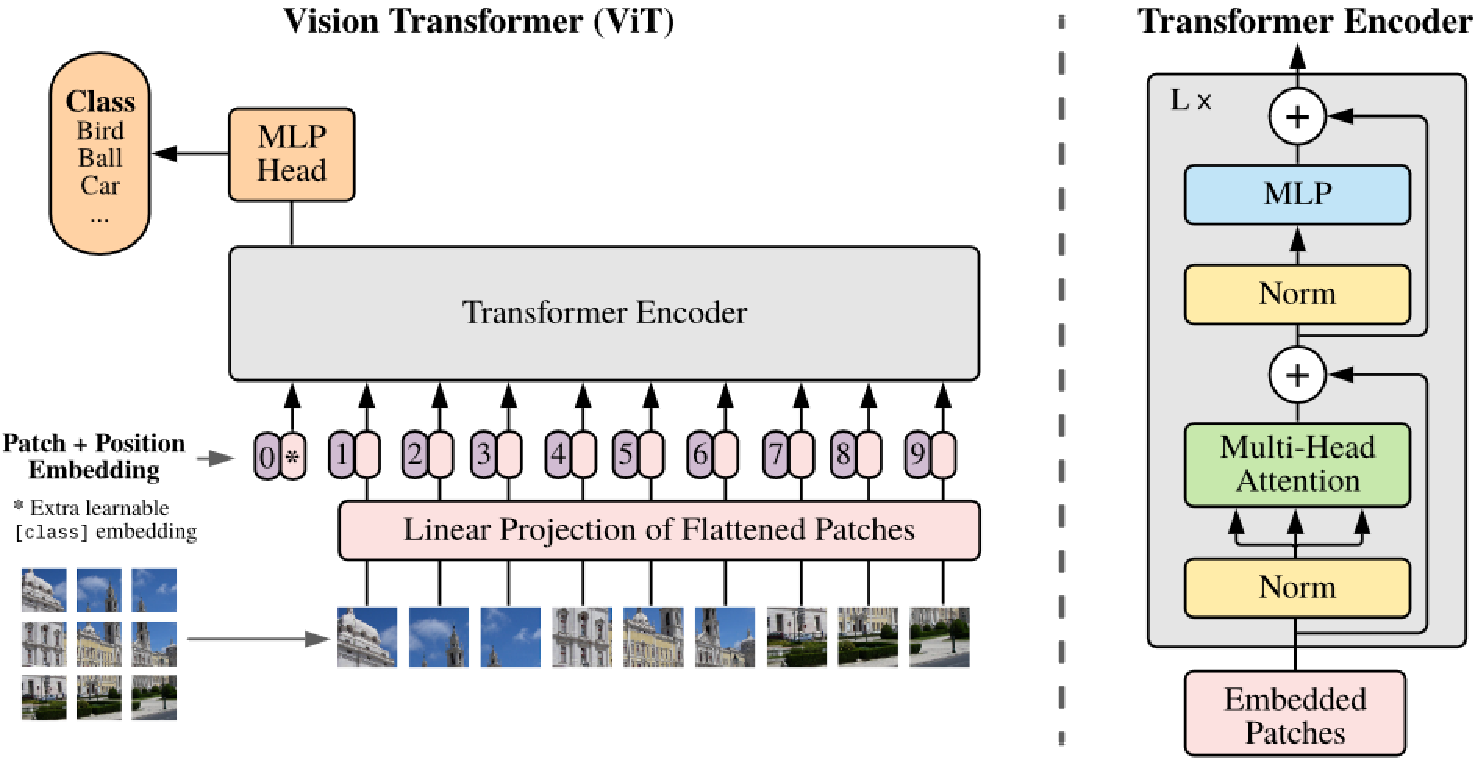
\includegraphics[width=145mm, height=76mm]{../img/VisualTransformerArchitecture}
\caption{Visual Transformer architecture from \citet{dosovitskiy2020image}.}
\label{fig01:ViT}
\end{figure}

\subsection{Decoder}
The second main part of the network is the decoder which serves as a language model for generating corresponding captions to input images. During the generation process the visual features of the image from the encoder and the already generated text are taken into account for the predtiction of the next token or word. In the process of generation, the attention mechanism (described above in the Chapter \ref{sec:methodsOfGeneration}) is almost always incorporated in order to focus only on the substantial particular areas. The following subsections presents common approaches used as the backbones for the decoder part of the network.
\subsubsection{Recurrent neural networks}
Recurrent neural networks (RNN)\footnote[2]{\url{https://en.wikipedia.org/wiki/Recurrent\_neural\_network}} are a category of neural networks designated for sequence data processing. Context of the previous part of the sequence can influnence the subsequent elements due to the RNN cell's internal memory (hidden state). Each time step RNN cell computes its activation function from current input and hidden state producing updated hidden state as output. For language modeling tasks, the last generated token or word is given to the RNN as the next input until the entire text is produced. The autoregressiveness of the RNNs is the reason why they are ideal for use as a language model. The two most used types of RNN cells are LSTM\citep{hochreiter1997long} and GRU\citep{cho2014learning}, however the LSTM cells are more utilized as the decoder because they can remember longer sequences. Moreover, we can combine them in a hierarchical manner to capture more complex structures in the generated text. Neverthless, the downside of the RNNs is the training time due to their sequential nature. The whole sentence must pass through RNN token by token and cannot be parallelized.

\subsubsection{GPT2}
Just as in the case of encoder, with the advent of transformers presented in the \citet{vaswani2017attention} paper, the deoder part of transformers started to be used as the language model for image captioning task for their great results in the natural language processing (NLP)\footnote[3]{\url{https://en.wikipedia.org/wiki/Natural\_language\_processing}} tasks. One of the advantages of the transformers against the previously used recurrent neural networks is the loss of the need for sequential processing during the training. Due to the fact that the processing of the whole caption can be done in parallel, the entire training process is significatnly accelerated. Moreover, the transformers can capture longer ranges dependencies in the text, as they process the sentence as a whole instead of sequentially by words.\\

One of the state-of-the-art autoregressive language models using transformers as their backbone is OpenAI GPT-2 model from the \citet{radford2019language} paper, which outperforms other language models on many NLP tasks. It was trained on a massive English dataset called WebText (introduced in the same article) containing a total of 40 GB of raw text. The resuling model is able to generate large coherent texts. Furthermore, it can be fine-tuned to a different domain or to a completely different language.

\section{Data}
In previous part we talked about possible methods of generation. Another crucial aspect we need to discuss are data, which are a basic building block of our thesis. This part focuses on the analysis of the data we used in our thesis, but also on their alternatives. \\

In order to solve our task and train neural network we need to get dataset containing the X-rays images along with their textual descriptions and optionally some other attributes of the examined X-rays. Moreover, the fundamental feature we need is that the data must be in the Czech language.

\subsection{Existing datasets}
\label{sec:datasets}
Medical environment provides a plenty of diverse potential problems, which can be researched. As already mentioned, in this thesis we focus specifically on the X-ray images. Because it is not so hard to detect fractures on the limbs, this area is not as interesting as others. One area that is rich in its diversity is the chest. As a result, this area is explored the most and therefore there exists multiple datasets with full textual mecidal reports. In the following section we describe some of them.\\

Apart from the datasets described below, other datasets with similar type are being used with the aim of solving our task. Amongst them belong datasets such as ImageCLEFmed~Caption\citep{ImageCLEFmedicalCaptionOverview2022}, PadChest\citep{bustos2020padchest}, BCIDR\citep{zhang2017mdnet} and PEIR~Gross\citep{jing2017automatic}. Moreover, except for datasets containing textual reports there exist a lot of other datasets worth mentioning containing different kind of information for each X-ray. These include, for example, CheXpert\citep{irvin2019chexpert}, VinDr-CXR\citep{nguyen2020vindr}, ChestX-ray8\citep{wang2017chestx} and its expanded version ChestX-ray14.

\subsubsection{Indiana University chest X-ray}
\label{sec:IUDataset}
Indiana University chest X-Ray dataset has become a standard in the field of medical report generation, it was presented in the \citet{10.1093/jamia/ocv080} paper. This dataset is an open source collection of pairs of chest X-rays and their corresponding semi-stuctured textual radiology reports, which is freely availble on the web\footnote[4]{\url{https://openi.nlm.nih.gov/faq\#collection}} without any additional requirements. We have a choice if we want to download just reports or images and in either PNG or DICOM format. The entire dataset consists of 7470 chest X-ray images that cover not only the frontal (PA\footnote[5]{Posterior-Anterior}) view, but also the lateral (side) one. These images corresponds to a total of 3995 patient's medical text reports.\\

Figure \hyperref[fig01:IUChestXRaySample]{1.1} shows an example from the Indiana University chest X-ray dataset. Each dataset pair is carefully de-identified in order to remove any personal information. The text of the report is semi-structured in up to 5 sections. The most important sections are \textit{impression}, where the overall diagnosis is stated, \textit{findings} section describing the details of examination and \textit{tags} which are of two types - manual and automatic. Manual tags were annotated manually using MeSH\footnote[6]{\url{https://www.nlm.nih.gov/mesh/meshhome.html}} and RadLex\footnote[7]{\url{http://radlex.org/}} codes, automatic were encoded from the reports using the MTI indexer. The rest of the sections are \textit{indication} and \textit{comparison}.\\

The disadvantage of this dataset is that it is relatively small. On the other hand, it is a clean and manually checked dataset containing also additional information about images in a form of tags described above.

\begin{figure}[h]\centering
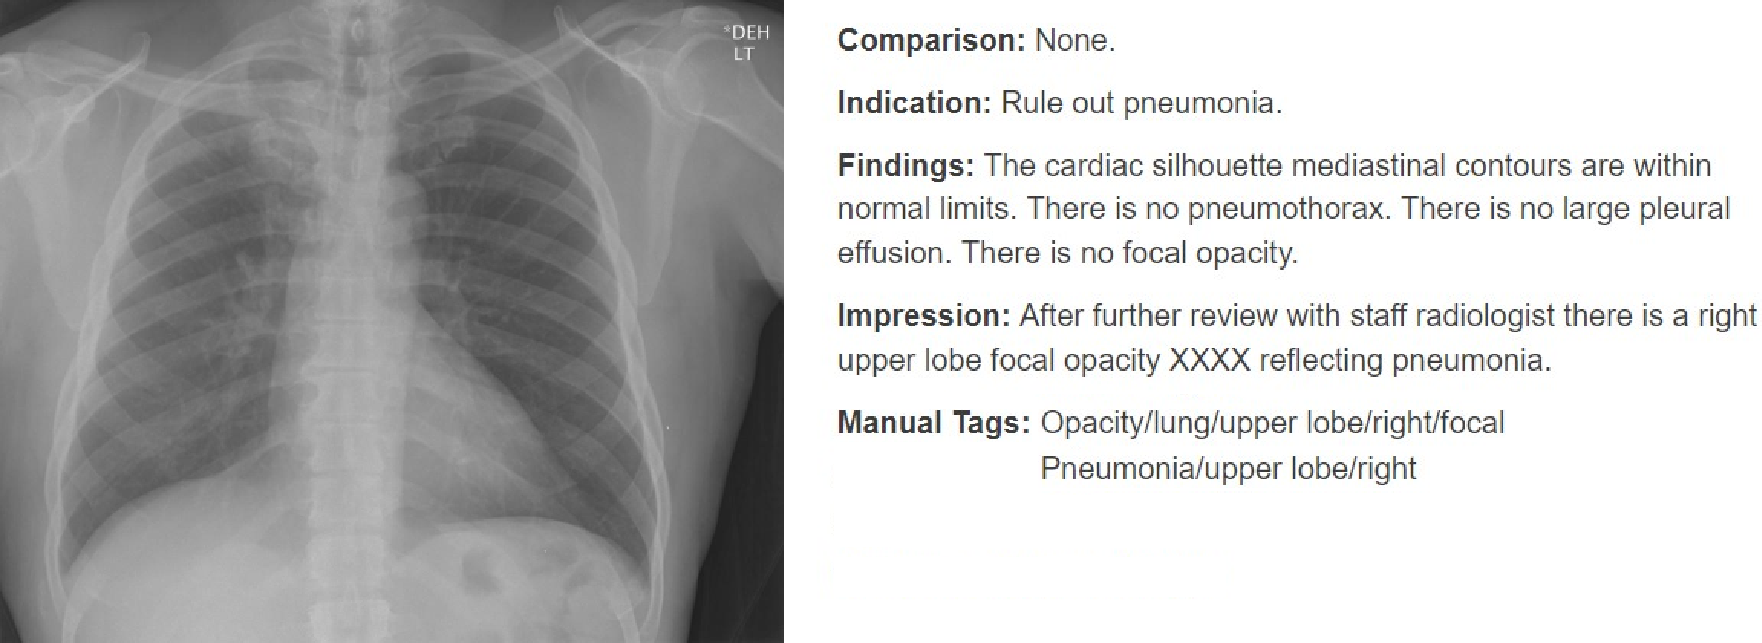
\includegraphics[width=145mm, height=53mm]{../img/IUChestXRaySample_CXR1728_IM-0479-1001}
\caption{Sample from the Indiana University Chest X-ray dataset.}
\label{fig01:IUChestXRaySample}
\end{figure}

\subsubsection{MIMIC-CXR v2.0.0}
MIMIC-CXR v2.0.0 is another dataset consisting of full semi-structured medical textual reports against corresponding chest X-rays that was presented in the \citet{cxr:johnson2019mimic} paper. As the previous dataset, it is openly available on the web\footnote[8]{\url{https://physionet.org/content/mimic-cxr/2.0.0/}}. In order to get access to the dataset, we have to go through registration and verification steps. The verification phase includes completion of CITI\footnote[9]{\url{https://about.citiprogram.org/series/human-subjects-research-hsr/}} \textit{Data or Specimens Only Research} course for \textit{Human Subject Research}. Moreover we need somebody trustworthy as a reference to confirm the authenticity of our identity. After the verification we get access to all datasets in the same repository.\\

The dataset consists of 377,110 X-ray images in the DICOM\footnote[10]{\url{https://www.dicomstandard.org/}} format connected to a total of 227,835 radiology reports for 65,379 patients. Each report is structured into multiple different sections. In order to satisfy legal requirements, entire dataset is automatically de-identified to remove any protected~health~information\footnote[11]{\url{https://en.wikipedia.org/wiki/Protected\_health\_information}}. Similalry to the previous dataset the essential two sections of each report are \textit{impression} and \textit{findings}. There also exists older MIMIC-CXR-JPG\footnote[12]{\url{https://physionet.org/content/mimic-cxr-jpg/2.0.0/}} dataset, presented in the \citet{cxr-jpg:johnson2019mimic} paper. This is an older version of MIMIC-CXR v2.0.0 dataset consisting of the exactly same images, only in JPG format, but each image is assigned 14 labels indicating the presence of the category in the report instead of its textual form. Each category has assigned either a \textit{1}, \textit{0} or \textit{-1} label with the meaning \textit{positively mentioned}, \textit{negatively mentioned} or \textit{uncertain}. The labels were determined from the reports utilizing the CheXpert\citep{irvin2019chexpert} and the NegBio\citep{peng2018negbio} open-source labelers.\\

The advantage of this dataset is its vast number of samples. Moreover, as described above, we can get additional information in a form of categories to every image. Nevertherless the textual reports carry some noise in them in the form of grammatical mistakes and incorrect formatting. We face these issues in the Chapter X. 

\begin{figure}[h]\centering
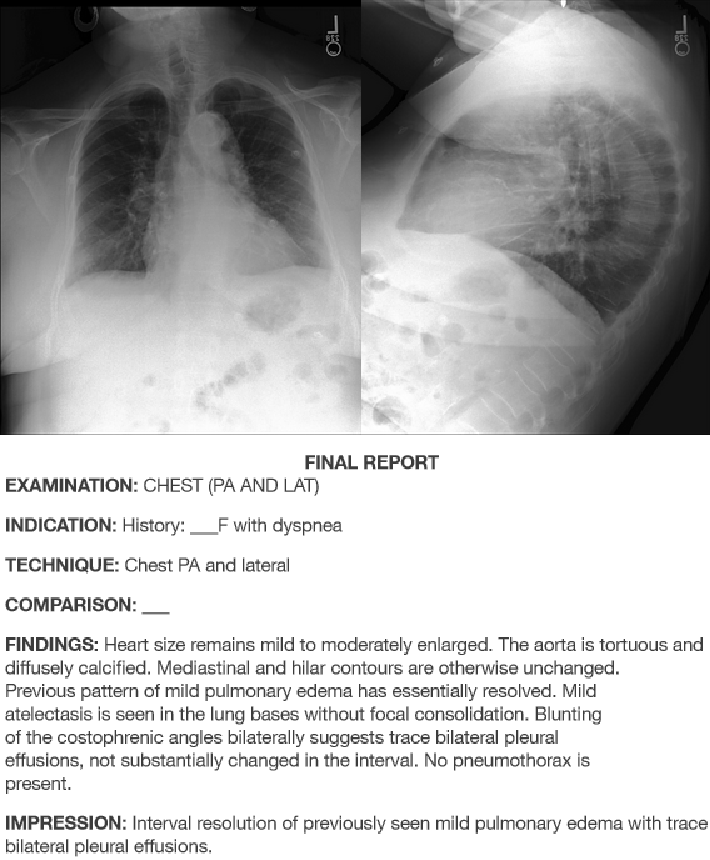
\includegraphics[width=135mm, height=163mm]{../img/mimic_s57861150}
\caption{Sample from the MIMIC-CXR dataset.}
\label{fig02:MimicCXRSample}
\end{figure}

\newpage

\subsection{Czech data}
All freely available datasets presented in the previous part have one common downside, namely they are not in the Czech language. As a part of elaboration of this thesis an intesive communication with real czech hospitals and other possible sources of real data took place. The goal of this communication was to create the very first open czech dataset of this kind. Processing of this kind of data would mean not only preparing the data into suitable format but also it would include proper anonymization of any personal information about the patients within the data. \\

However, inasmuch as the authentic patients data from hospitals are subject to strict privacy rules and we are not employees of any hospital, the institutions decided that they cannot provide the data in any way without the concious permission of patients given before the examination. With this result we need to find a different way how to obtain this much needed czech data.

\subsection{Translators}
In the previous sections we discovered that there is no dataset in the Czech language for our problem and there is no easy way how to get acces to the real data in order to build one. The only thing left is to create a new artificial dataset using an automatic translation. We will compare different freely accesible translators and choose the right one for our needs.

\subsubsection{DeepL}
At the moment, DeepL\footnote[13]{\url{https://www.deepl.com/translator}} translator provides the finest available translations beating even the ones from Google Translate. Moreover, it has freely usable web application and REST API. However, the main drawback of the DeepL translator is that its REST API is highly limited - only 500 000 characters per month can be translated for free. Furthermore, any translation above this limit is costly and thus this path is not appropriate for translating large textual datasets. One way to get around this problem is to use their internal REST API used specifically for the web application, which is free to use. We investigated and implemented this potential way in our thesis and further experimented how much it can be used, but unfortunately even this internal REST API is strictly limited for only tens of consecutive\footnote[14]{REST API calls are delayed from each other for some time, otherwise the service is blocked immediately} translations making it unusable for out needs.

\subsubsection{Google Translate}
Google~Translate\footnote[15]{\url{https://translate.google.com/}} has become already de facto standard in the world of machine translation and it is the most used freely accessible language translation service in the world. In terms of quality, the translations are still great although little bit worse than those from DeepL. The web application is free of any charge and anybody can use it as much as he needs. Nevertheless, just as in the case of DeepL, their REST API services are limited and translation of anything above that limit is expensively charged. For these reasons, as in the previous case, we must find another way.

\subsubsection{CUBBITT}
Machine~Translation\footnote[16]{\url{https://en.wikipedia.org/wiki/Machine\_translation}} is an extensive area of research, as a result of which there exist many other projects and academic papers nowadays. One of them is CUBBITT\footnote[17]{\url{https://lindat.mff.cuni.cz/services/translation/}} translator, which was developed at our faculty. The whole system is presented and described in detail in the \citet{biblio:PoToTransformingmachine2020} paper. \\

CUBBITT translator provides translations which are comparable to the ones from DeepL and Google Translate services. As other mentioned translators it provides an openly available web application for machine translation. Moreover and most importantly it provides REST API that is completely unlimited in text volume and free to use without any additional charges. These are the reasons why we will utilize CUBBITT in our thesis as a translator to create our artificial dataset.\\

On the other hand, CUBBITT has not support for auto-correcting input text compared to above mentioned services. Moreover, there are some patterns in the text which CUBBITT cannot translate at all or translates them incorrectly. These problems complicates our situation as the data from hospitals carry some natural noise in them. We face these complications in Chapter X.

\section{Related work}
\label{sec:RelatedWork}
The last section of this chapter is dedicated to the description and comparison to some of the related works that solves identical or similar problem as we do.\\

The most significant related work is \citet{alfarghaly2021automated} inasmuch as we base our thesis on it. This paper focuses on the identical problem as we do, only in the English language. The proposed solution uses a pre-trained and further fine-tuned Chexnet model, presented in \citet{rajpurkar2017chexnet}, as a visual features encoder and distilGPT2 language model\citep{radford2019language} as a decoder which is additionally conditioned on the visual features and predicted tag's word2vec\citep{mikolov2013distributed} embeddings. For training the neural network the Indiana University chest X-ray dataset, described in more detail in Chapter \ref{sec:IUDataset}, is used. Figure \hyperref[fig03:OmarExample]{1.3} shows examples of the model outputs.\\

\begin{figure}[h]\centering
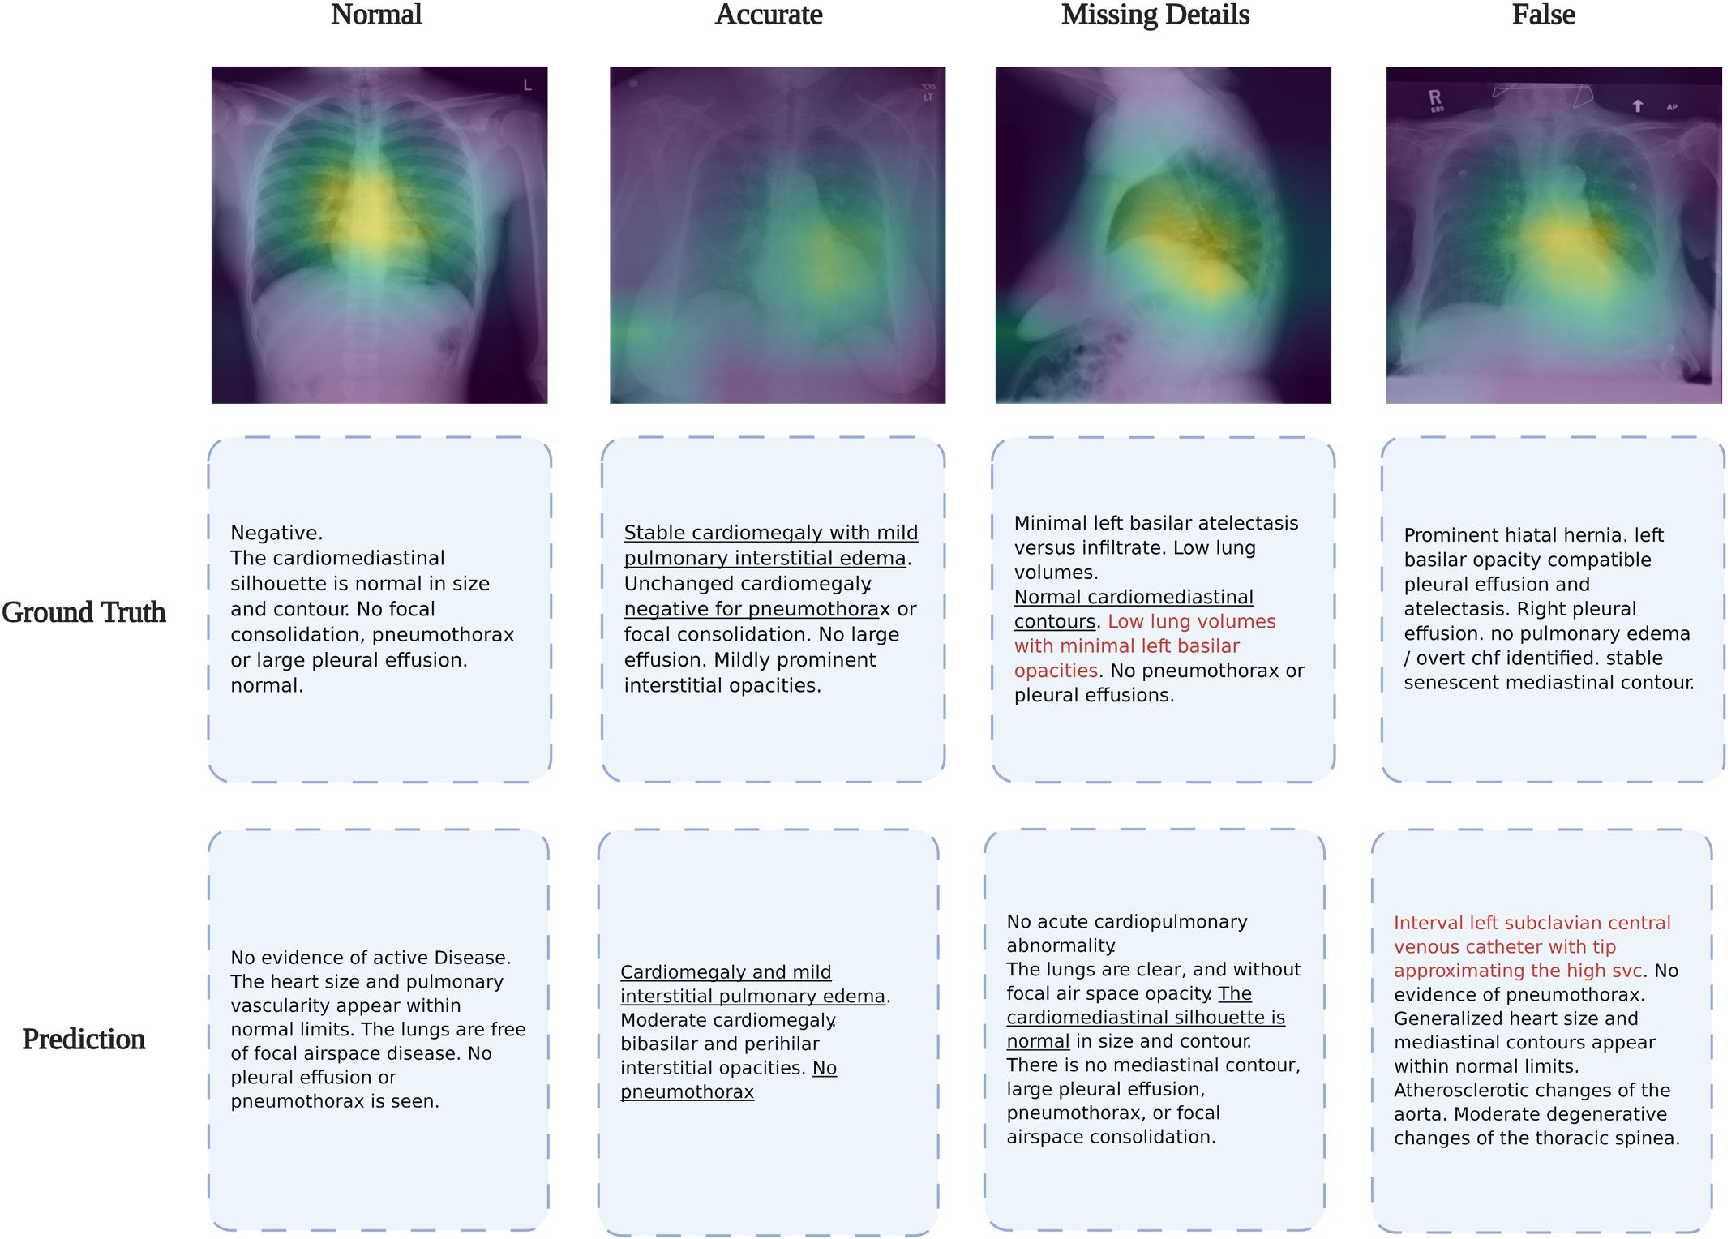
\includegraphics[width=145mm, height=104mm]{../img/OmarExample}
\caption{Examples of generated medical reports from \citet{alfarghaly2021automated}.}
\label{fig03:OmarExample}
\end{figure}

Another paper making use of transformers is \citet{chen2020generating}. The visual features of images are extracted using pre-trained convolutional neural network and they are further passed to the transformer encoder outputting hidden states, that are further presented to the transformer decoder for the report generation. However, the decoder architecture contains special memory module and also enhances the layer normalization. The memory module serves for memorization of text patterns which occur in the similar images inasmuch as they can further help for generating the report. We can see its effect in the Figure \hyperref[fig04:ZhihongExample]{1.4}. Indiana University chest X-ray and MIMIC-CXR v2.0.0 datasets (see Chapter \ref{sec:datasets} for more details) were used as training data.\\

\begin{figure}[h]\centering
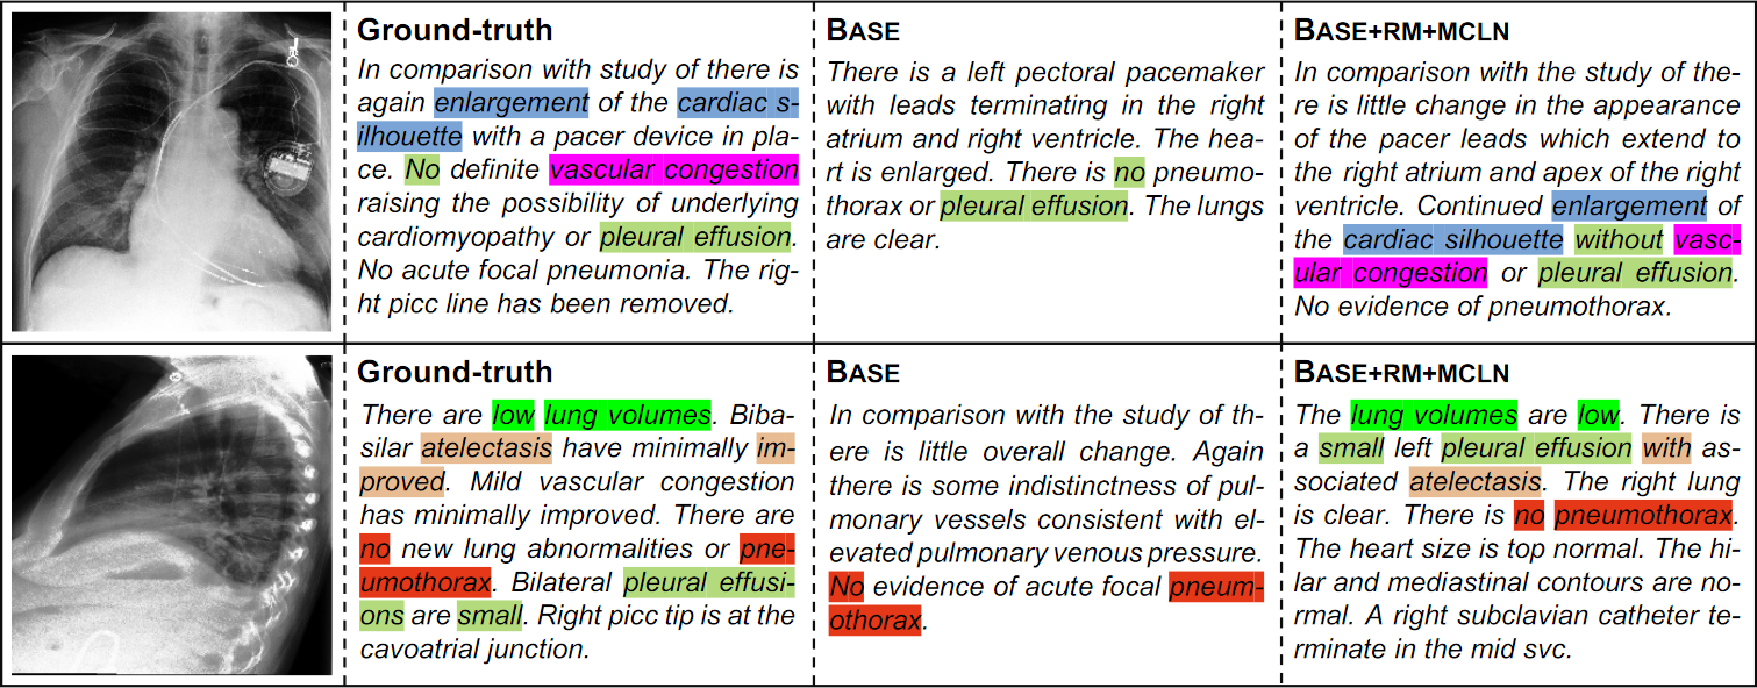
\includegraphics[width=145mm, height=57mm]{../img/ZhihongExample}
\caption{Examples of generated medical reports from \citet{chen2020generating}.}
\label{fig04:ZhihongExample}
\end{figure}

\citet{yuan2019automatic} paper proposes a hiearchical encoder-decoder architecture as we can see in the Figure \hyperref[fig05:YuanExample]{1.4} for the purpose of generating textual reports. Pairs of frontal and lateral X-ray images are used as an input to the network instead of single images, as the authors claim that the images should be complementary to each other instead of being processed independently. The RestNet-152 model pre-trained on the CheXpert\citep{irvin2019chexpert} dataset is utilized as the encoder with three outputs used later - the global and local features of the images, predticted observations and medical concepts. The decoder is hierarchical LSTM decoder comprising of the two parts: \textit{sentence decoder} and \textit{word decoder}. The sentence decoder takes visual features and generates hidden state for each sentence, which are along with the predicted medical concepts presented to the word decoder in order to generate the report. There are many other papers using a hierarchical architecture, e.g. \citet{huang2019multi}. \\

\begin{figure}[h]\centering
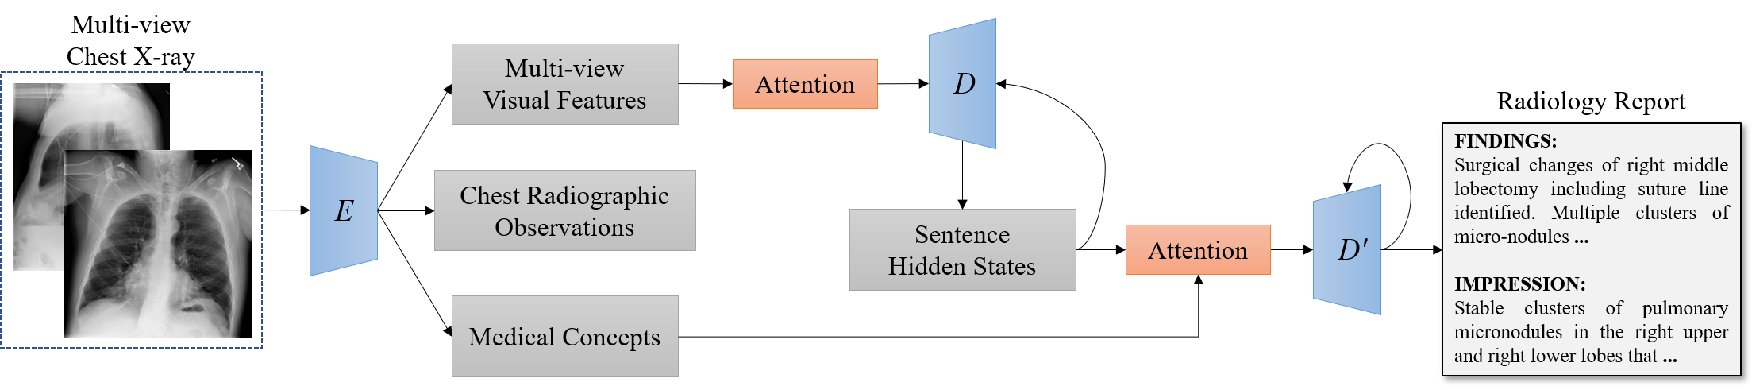
\includegraphics[width=145mm, height=32mm]{../img/YuanExample}
\caption{Hierarchical architecture from \citet{yuan2019automatic}.}
\label{fig05:YuanExample}

\textit{E} is encoder, \textit{D} is sentence decoder and \textit{D\textquotesingle} is word decoder.
\end{figure}

The last related project we mention in this work is CareBot\footnote[18]{\url{https://www.carebot.com/}}, which is being developed concurrently with our thesis. CareBot is a czech startup founded in 2021 as a reaction to the then ongoing Covid-19 pandemic. As in our work, CareBot focuses its attention mainly on the processing of chest X-rays using neural networks. However, unlike us it does not generate the textual reports for the doctors. Instead of textual reports, it focuses on finding and classifying a total of 15 different types of individual diseases on X-ray images and their subsequent spatial localization. Moreover, they already have a support from the medical environment.












\chapter{Title of the second chapter}

\section{Title of the first subchapter of the second chapter}

\section{Title of the second subchapter of the second chapter}

\chapter{Experiments}
This chapter describes all the experiments we conducted during the elaboration of our thesis and which will be further evaluated in the following chapter. Moreover, we will some describe technical details, scripts and environments we used for our experiments. The entire code is written in Python 3 with the use of tensorflow\footnote[1]{\url{https://www.tensorflow.org/}}, pyTorch\footnote[2]{\url{https://pytorch.org/}}, huggingface\footnote[3]{\url{https://huggingface.co/}} and fastai\footnote[4]{\url{https://www.fast.ai/}} libraries as they are the standard for working with neural networks. To install all the required dependencies, run the following command in the appropriate part of the project:

 \begin{code}
> pip3 install -r requirements.txt
\end{code}

\section{Environment}
For training our neural networks, we used two different computational clusters, namely - AIC cluster\footnote[5]{\url{https://aic.ufal.mff.cuni.cz/index.php/Main\_Page}} and IT4I cluster.\footnote[6]{\url{https://www.it4i.cz/}} Both of them provide a support fo CPU and GPU computational tasks. However, since our models are large, we only train on GPUs.  For less time-consuming tasks, especially in the earlier phases of our thesis, we employed the AIC cluster. The IT4I cluster was used for the final training of all our models and all values reported in the subsequent parts of the text refer to the IT4I cluster hardware. Table \ref{tab01:clusterHW} lists the hardware available in both clusters.

\begin{table}[h]
\centering
\begin{tabular}{l@{\hspace{0.75cm}}D{.}{,}{0}D{.}{,}{5.0}D{.}{,}{1.2}}
\toprule
 & \mc{} & \mc{} \\
\pulrad{\textbf{Cluster}} & \mc{\pulrad{\textbf{GPU}}} & \mc{\pulrad{\textbf{Memory}}}\\
\midrule
AIC                  & \mc{NVIDIA GeForce GTX 1080 Ti}  & \mc{11 GB}\\
IT4I                 & \mc{NVIDIA A100 SXM4 40GB} & \mc{40 GB}\\
\bottomrule
\multicolumn{3}{l}{\footnotesize \textit{Note:} Clusters provide multiple types of GPUs. Only the types used are listed.}
\end{tabular}

\caption{Available GPU hardware on clusters.}\label{tab01:clusterHW}
\end{table}

\section{Czech GPT-2}
\label{sec:gpt2Experiments}
This section summarizes all experiments, results and scripts related to the training of Czech GPT-2 models. All training experiments were performed according to the mind description in Chapter \ref{sec:czechGpt2}. Scripts related to the GPT-2 training and subsequent work are prefixed with \textit{gpt2}.\\

During the elaboration of this thesis, we trained a several GTP-2 models on different datasets and with different approaches. However, we present only the most important results as we are interested only in the best possible GPT-2 models.\\

The learning rates for both models were determined using the approach described in Chapter \ref{sec:gpt2Training}. For the general Czech GPT-2 model, the learning rates of $4e^{-3}$ for the first phase of learning only the new head and $2e^{-3}$ for the training of the entire unfrozen model were used. Subsequent fine-tuning of the medical model was performed using the learning rates of $8e^{-4}$ and $4e^{-4}$. Both of the models use batch size of 16 as it is the maximum that could fit into the GPU and sequence length of 512 for the reasons discussed in the mentioned chapter. Entire training of each of the models took a total of 5 epochs.

\subsection{Implementation}
The implementation of the GPT-2 related part comprises of several scripts. This section describes all of them with the necessary level of detail.

\subsubsection*{Training}
The most important script is \textit{gpt2\_train.py} that takes care of the entire training process. The script is parametrized with a numerous arguments such as base GPT-2 model, required sequence length, path to data etc. The data are expected to be inside the \textit{storage/data} directory. In the beginning, the script creates all directories necessary for the training and its results - this includes the directories for the final model, checkpoints, intermediate training data and tokenizers. After the initialization, the script runs according to the description of the process in Chapter \ref{sec:gpt2Training}. Further, the script also allows to resume the training from the last saved checkpoint. Final trained model is saved in both tensorflow and pyTorch version at the end along with its corresponding tokenizer in the \textit{storage/models} directory. Description of all arguments, that can be entered at the input, is directly inside the script. The script can be run as follows:
\begin{code}
> python3 gpt2_train.py [-h] [--type {gradual,full}] 
                [--model MODEL] [--max_len MAX_LEN] 
                [--pretrained_weights PRETRAINED_WEIGHTS] 
                [--dataset DATASET] [--data_path DATA_PATH] 
                [--batch_size BATCH_SIZE]
                [--train_data_ratio TRAIN_DATA_RATIO] 
                [--sequence_length SEQUENCE_LENGTH] [--debug DEBUG] 
                [--resume_training RESUME_TRAINING] 
                [--find_learning_rates FIND_LEARNING_RATES]
                [--pretokenize_data PRETOKENIZE_DATA] 
                [--save_checkpoints SAVE_CHECKPOINTS] 
                [--learning_rates LEARNING_RATES [LEARNING_RATES ...]]
\end{code}
\newpage

\subsubsection*{Testing}
The \textit{gpt2\_generate.py} script serves for the text generation purposes. It is applicable to any huggingface GPT-2 model whose model name or path is taken as an argument. Moreover, all parameters that can be passed to the general huggingface GPT-2 \textit{generate} method can be also passed as arguments of the script such as \textit{top\_p}, \textit{top\_k} etc. The ouput of the script is the texts generated by the given GPT-2 model. The script can be run as follows:
\begin{code}
> python3 gpt2_generate.py [-h] [--max_len MAX_LEN] 
                          [--model MODEL] 
                          [--top_k TOP_K] 
                          [--top_p TOP_P] 
                          [--repetition_penalty REPETITION_PENALTY] 
                          [--temperature TEMPERATURE] 
                          [--do_sample DO_SAMPLE]
                          [--num_return_sequences NUM_RETURN_SEQUENCES]
\end{code}

\subsubsection*{Data preparation}
The last important script is \textit{gpt2\_data\_utils.py}. As the \textit{gpt2\_train.py} script needs the data to be in a specific format, this script provides tools for their preparation. For the specified data location, it goes through all files with \textit{.txt} or other user specified extensions. Each of the files can be further split after each number of lines or by a given delimiter. Finally, two files are created- one \textit{.txt} file with all texts merged inside the file for the tokenizer training and one \textit{.csv} file, where each split part corresponds to one row, for the GPT-2 fine-tuning itself. The script can be run as follows:\\
\begin{code}
> python3 gpt2_data_utils.py [-h] [--folder FOLDER] 
                             [--text_delim TEXT_DELIM] 
                             [--regenerate REGENERATE] 
                             [--line_split LINE_SPLIT] 
                             [--extensions EXTENSIONS]
\end{code}

For the OSCAR dataset (and generally any other dataset from huggingface), we implemented the \textit{DatasetsWrapper} class encapsulating the huggingface datasets classes, that provides us with better data handling, direct text iteration, control character filtering and offers us the ability to save data directly to a specified file while preserving all the original functionality. The class is implemented in the \textit{datasets\_wrapper.py} file.

\subsection{Results}
In this section, we present the training results for our fine-tuned Czech GPT-2 models. The trainig results can be seen in Table \ref{tab02:GeneralCzGpt2Results} and Table \ref{tab03:MedicalCzGpt2Results}. During training, we measured accuracy and perplexity\footnote[7]{\url{https://en.wikipedia.org/wiki/Perplexity}} metrics.

We can see that the general model achieved an accuracy of 40.02 and a perplexity of 30.35. These values are comparable to the original article, where they trained a model for Portuguese. However, there are two major differences between ours and theirs setup. First, our training was conducted on a total of a 21 GB of raw data, compared to the original 1.6 GB. Further, we train our model on sequences of length 512 compared to original 1024. Both of these factors decrease our measured values and thus the results cannot be compared directly. Nevertheless, even if we trained the model with an identical sequence length, our results would be worse than in the original paper even though we trained on an order of magnitude larger data. This is due to the fact that Portuguese and English are more similar languages and because the original article used only more homogenous data from Wikipedia.\\

As for the specialized medical GPT-2 model, the results are almost identical to the general Czech GPT-2 model. The fine-tuning was really fast as each epoch took  a maximum of 10 minutes. Nevertheless, we could get even better results, if we had better and more extensive Czech medical data to train the model for a longer period of time.

\begin{table}[h!]

\centering
\begin{tabular}{l@{\hspace{0cm}}D{.}{,}{0}D{.}{,}{1.2}D{.}{,}{1.2}D{.}{,}{2.2}D{.}{,}{2.2}D{.}{,}{1.2}D{.}{,}{2.2}}
\toprule
 & \mc{} & \mc{} & \mc{} & \mc{} & \mc{} & \mc{} & \mc{} \\
\pulrad{\textbf{Epoch}} & \mc{\pulrad{\textbf{Loss\textsubscript{train}}}} & \mc{\pulrad{\textbf{Loss\textsubscript{val}}}} & \mc{\pulrad{\textbf{Accuracy (\%)}}} & \mc{\pulrad{\textbf{Perplexity}}} & \mc{\pulrad{\textbf{Time (h)}}} \\
\midrule
\mc{1}                & \mc{4.42}          & \mc{4.28}  & \mc{30.40} & \mc{72.10} & \mc{26:56} \\
\mc{2}                & \mc{3.75}          & \mc{3.76}  & \mc{35.99} & \mc{42.85} & \mc{29:07} \\
\mc{3}             	  & \mc{3.74}          & \mc{3.65}  & \mc{37.20} & \mc{38.32} & \mc{29:07} \\
\mc{4}                & \mc{3.61}          & \mc{3.54}  & \mc{38.48} & \mc{34.38} & \mc{28:58} \\
\mc{5}                & \mc{3.52}          & \mc{3.41}  & \mc{40.02} & \mc{30.35} & \mc{28:57} \\
\bottomrule
\multicolumn{7}{l}{\footnotesize \textit{Note:} All values are rounded to 2 decimal places.}
\end{tabular}

\caption{General Czech GPT-2 model training results.}\label{tab02:GeneralCzGpt2Results}
During the first epoch, only the new head is trained.
\end{table}

\begin{table}[h!]

\centering
\begin{tabular}{l@{\hspace{0cm}}D{.}{,}{0}D{.}{,}{1.2}D{.}{,}{1.2}D{.}{,}{2.2}D{.}{,}{2.2}D{.}{,}{1.2}D{.}{,}{1.2}}
\toprule
 & \mc{} & \mc{} & \mc{} & \mc{} & \mc{} & \mc{} & \mc{} \\
\pulrad{\textbf{Epoch}} & \mc{\pulrad{\textbf{Loss\textsubscript{train}}}} & \mc{\pulrad{\textbf{Loss\textsubscript{val}}}} & \mc{\pulrad{\textbf{Accuracy (\%)}}} & \mc{\pulrad{\textbf{Perplexity}}} & \mc{\pulrad{\textbf{Time (m)}}} \\
\midrule
\mc{1}                & \mc{3.85}          & \mc{3.75}  & \mc{35.90} & \mc{42.42} & \mc{9:01} \\
\mc{2}                & \mc{3.74}          & \mc{3.66}  & \mc{36.76} & \mc{38.90} & \mc{9:50} \\
\mc{3}             	  & \mc{3.63}          & \mc{3.52}  & \mc{38.58} & \mc{33.62} & \mc{9:49} \\
\mc{4}                & \mc{3.41}          & \mc{3.43}  & \mc{39.94} & \mc{30.75} & \mc{9:48} \\
\mc{5}                & \mc{3.14}          & \mc{3.41}  & \mc{40.29} & \mc{30.36} & \mc{9:48} \\
\bottomrule
\multicolumn{7}{l}{\footnotesize \textit{Note:} All values are rounded to 2 decimal places.}
\end{tabular}

\caption{Medical Czech GPT-2 model training results.}\label{tab03:MedicalCzGpt2Results}
During the first epoch, only the new head is trained.
\end{table}

\subsection{Examples}
In the last part of the GPT-2 experiments section, examples of texts generated by both of the trained models are shown and further discussed.

\subsubsection*{General Czech GPT-2}
TODO
\subsubsection*{Medical Czech GPT-2}
TODO

\section{Dataset translation}
Medical dataset translation is a large part of the thesis. This section describes all necessary details of the data translation. As our final data source we chose the Indiana University chest X-ray dataset and we utilized CUBBITT as the translation service. Implementation details for all related source code are described below. Processing of the whole dataset (3955 files) took a total of 32 minutes.

\subsection{Implementation}
To translate medical reports from English into Czech, the \textit{dataset\_translate.py} script was utilized. It is designed to be versatile and extensible for use on any dataset and any translation service. One can define its own \textit{Translator} or \textit{Extractor} class, described in the following parts of text, and run the script with different data or translator. Moreover, the preprocessing pipeline can also be customized to specific requirements. The script can be run as follows: \\
\begin{code}
> python3 dataset_translate.py [-h] [--translator {cubbitt,deepl}] 
                               [--dataset {mimic,openi}] 
                               [--data DATA]
                               [--preprocess {lowercase,pipeline,none}] 
                               [--preprocess_only PREPROCESS_ONLY]
                               [--anonymous_seq ANONYMOUS_SEQ]
\end{code}

It takes several arguments, such as the data path, and runs the translation. The script runs in multiple threads, so it can make efficient use of system resources and therefore speed up the overall translation. The final report translations are stored in the \textit{translations} directory, where each run is uniquely identified by its start date, dataset name etc., while preserving the original dataset structure. If the user do not want to translate the dataset and only preprocess, the behaviour of the script can be changed with the \textit{--preprocess\_only} argument.\\

For each file, the script first loads the report text using the specified \textit{Extractor}. Next, the text goes through each of the \textit{Preprocessors} to process the text. After the preprocessing finishes, the report is passed to the selected \textit{Translator} to get the translated text. Finally, the translated report is saved under the original file name. Throughout the entire translation process, the progress indication of how much data has been already translated is displayed.\\

All implemented preprocessors, described in Chapter\ref{sec:DataPreprocessing}, are located in the \textit{preprocessors} directory. Each of them implements the  \textit{Preprocessor} interface with only one method \textit{preprocess}, which makes it extensible for possible additional user defined preprocessors.\\

In our thesis we utilize CUBBITT as our translator. However, the user can implement its own translator class as the main script for dataset translation works with \textit{Translator} interface. This interface defines two methods - \textit{translate} that should return the response object from the translation service, and \textit{get\_text} that should get or create the translated text from the response. During the elaboration of this thesis we also implemented a translator for the DeepL, but it is unusable in practice due to its strict limits.

The last extensible part of the translation process is text extraction from the dataset files. Since not all datasets are just simple \textit{.txt} files, we created the \textit{Extractor} interface for this purpose. It defines only one method \textit{extract\_report} intended for full report text extraction. We implemented two extractors - for the Indiana University chest X-ray and MIMIC-CXR v2.0.0 datasets.

\section{Medical report generation model}
Tha last section of this chapter describes all the experiments conducted for the medical report generation. Furthermore, all the necessary technical information about running models and data preparation is summarized.

\subsection{Setup}
As we already mentioned in the previous parts of text, we use the solution from \citet{alfarghaly2021automated} paper that is freely available on the github.\footnote[8]{\url{https://github.com/omar-mohamed/GPT2-Chest-X-Ray-Report-Generation}} The code uses older tensorflow 2.3.0 with some deprecated features, thus some minor adjustments had to be done in order to run on a newer 2.5.0 version. This version wss chosen because of the available support for the corresponding CUDA and cuDNN version on the IT4I cluster. \\

For the training, the Inidiana Univesity chest X-ray dataset was utilized as in the original paper. The key reason is that the solution uses a pre-trained CNN backbone, which is directly fine-tuned for the Inidiana Univesity chest X-ray dataset tags. The MIMIC-CXR v2.0.0 does not provide these tags, but only 14 labels. Thus the original Chexnet model would have to be fine-tuned again for this huge dataset. Morevoer, the whole training time would be considerably prolonged and the code would have to be modified more extensively\\.
 
As we need to have the Czech translated reports in the same format as in the original case, we implemented a script to do so. The reports contain several sections, however for the final report training and prediction, only the \textit{Impression} and \textit{Findings} sections are taken as they contain key information. The script for the modification of the original \textit{csv} files can be run as follows:
\begin{code}
> python3 modify_csv_to_translations.py [-h] 
                                [--original_csv_dir ORIGINAL_CSV_DIR] 
                                [--translations_dir TRANSLATIONS_DIR]
                                [--output_dir OUTPUT_DIR]
\end{code}

First, follow the setup steps described in the project \textit{README}. Next, in order to run a training for our GPT-2 models and Czech data, several steps need to be carried out:
\begin{itemize}
	\item In the \textit{IU-XRay} directory, the English report files must be swapped with their Czech translations - \textit{all\_data.csv}, \textit{testing\_set.csv}, \textit{training\_set.csv}.
	\item The desired trained GPT-2 model should be placed inside the top level of the directory.
	\item Inside the \textit{train.py}, \textit{test.py}, \textit{tokenizer\_wrapper.py} files, the original distilgpt2 and gpt2 model and tokenizer string identifier should be changed to the name of our trained GPT-2 model.
	\item Change hyperparameters in \textit{configs.py} to adjust training parameters as needed.
\end{itemize}

After all the mentioned steps, we can run the training or testing procedure using the following commands:
\begin{code}
> python3 train.py
> python3 test.py
\end{code}

\subsection{Experiments}
Final thing that needs to be perfomed is to run experiments for the medical report generation. We conducted our experiments with multiple different setups of the neural network. All of them were performed on the IT4I cluster with the batch size of 8 as it was the maximum size we were able to fit into the GPU. In the original article, they trained the model with the constant learning rate of $1e^{-3}$ and Adam optimizer. Nevertheless, we trained our models with a smaller learning rate of $1e^{-4}$, because we find it better to train already pre-trained models with a lower value. The max sequence length is set to be 200 tokens, as the reports are generally shorter nature.\\

We run the final training on both of our trained Czech GPT-2 models - general Czech model and specialized Czech medical model. On top of the original paper where they trained only the decoder part of the network with the frozen CNN backbone, we also train with setups in which we have left the entire network unfrozen. In the end, we have a total of 4 different setups listed in Table \ref{tab04:MedGenReportSetups} for training. For each of them, the best and the last model will be evaluted.

\begin{table}[h!]
\centering
\begin{tabular}{l@{\hspace{0.75cm}}D{.}{,}{7.0}D{.}{,}{4.0}}
\toprule
 & \mc{} & \mc{} \\
\pulrad{\textbf{Model}} & \mc{\pulrad{\textbf{Training scope}}} & \mc{\pulrad{\textbf{Identifier}}} \\
\midrule
General Czech GPT-2               & \mc{Decoder only}          & \mc{GEN-dec}  \\
General Czech GPT-2               & \mc{Entire network}        & \mc{GEN-all}  \\
Medical Czech GPT-2               & \mc{Decoder only}          & \mc{MED-dec}  \\
Medical Czech GPT-2               & \mc{Entire network}        & \mc{MED-all}  \\
\bottomrule
\multicolumn{3}{l}{\footnotesize \textit{Note:} Tags' embeddings are frozen during all setups.}
\end{tabular}

\caption{Medical report generation experiments' setups.}\label{tab04:MedGenReportSetups}
\end{table}



\chapter{Experiments}
This chapter describes all the experiments we conducted during the elaboration of our thesis and which will be further evaluated in the following chapter. Moreover, we will describe some technical details and environments we used for our experiments.\\

In the beginning, we want to emphasize the fact that during the elaboration of this thesis we performed a lot of experiments with different setups, methods, and data. Nevertheless, we present only the experiments and setups we used for the final experiments and evaluation.

\section{Environment}
For training our neural networks, we used two different computational clusters, namely - AIC cluster\footnote[1]{\url{https://aic.ufal.mff.cuni.cz/index.php/Main\_Page}} and IT4I cluster.\footnote[2]{\url{https://www.it4i.cz/}} Both of them provide support for CPU and GPU computational tasks. However, since our models are large, we perform the trainings only on GPUs.  For less time-consuming tasks, especially in the earlier phases of our thesis, we employed the AIC cluster. The IT4I cluster was used for the final training of all our models and all values reported in the subsequent parts of the text refer to the IT4I cluster hardware. Table \ref{tab01:clusterHW} lists the hardware available in both clusters. This work was supported by the Ministry of Education, Youth and Sports of the Czech Republic through the e-INFRA CZ (ID:90140)

\begin{table}[h]
\centering
\begin{tabular}{l@{\hspace{0.75cm}}D{.}{,}{0}D{.}{,}{5.0}D{.}{,}{1.2}}
\toprule
 & \mc{} & \mc{} \\
\pulrad{\textbf{Cluster}} & \mc{\pulrad{\textbf{GPU}}} & \mc{\pulrad{\textbf{Memory}}}\\
\midrule
AIC                  & \mc{NVIDIA GeForce GTX 1080 Ti}  & \mc{11 GB}\\
IT4I                 & \mc{NVIDIA A100 SXM4 40GB} & \mc{40 GB}\\
\bottomrule
\multicolumn{3}{l}{\footnotesize \textit{Note:} Clusters provide multiple types of GPUs. Only the types used are listed.}
\end{tabular}

\caption{Available GPU hardware on clusters.}\label{tab01:clusterHW}
\end{table}

\section{Czech GPT-2}
\label{sec:gpt2Experiments}
This section summarizes all experiments and results related to the training of Czech GPT-2 models. All experiments were performed according to the training procedure description in Chapter \ref{sec:gpt2Training}.\\

During the elaboration of this thesis, we trained several GPT-2 models on different datasets and with different approaches. Specifically, in addition to experiments described below, we performed training on many different learning rates given by the learning rate finding procedure. Experiments were done for all datasets described in Chapter \ref{sec:gptData}. Furthermore, the original gradual unfreezing training procedure was another part that was experimented with. However, we present only the most important results as we are interested only in the best possible GPT-2 models.\\

The learning rates for both models were determined using the approach described in Chapter \ref{sec:gpt2Training}. For the general Czech GPT-2 model, the learning rates of $4e^{-3}$ for the first phase of learning only the new head and $2e^{-3}$ for the training of the entire unfrozen model were used on the OSCAR dataset. Subsequent fine-tuning of the medical model was performed using the learning rates of $8e^{-4}$ and $4e^{-4}$ respectively. Both of the models use a batch size of 16 as it is the maximum that could fit into the GPU and sequence length of 512 for the reasons discussed in the referenced chapter. The entire training of each of the models took a total of 5 epochs. After some experimenting with the number of training epochs, we concluded that additional epochs do not bring any significant improvement. Overview of hyperparameters used for each model training is given in Table \ref{tab00:Gpt2TrainingParams}.

\begin{table}[h!]
\centering
\begin{tabular}{l@{\hspace{0cm}}D{.}{,}{0}D{.}{,}{1.3}D{.}{,}{1.3}D{.}{,}{2.0}D{.}{,}{3.0}D{.}{,}{1.0}}
\toprule
 & \mc{} & \mc{} & \mc{} & \mc{} & \mc{} & \mc{} \\
\pulrad{\textbf{Model}} & \mc{\pulrad{\textbf{LR\textsubscript{Head}}}} & \mc{\pulrad{\textbf{LR\textsubscript{All}}}} & \mc{\pulrad{\textbf{Batch size}}} & \mc{\pulrad{\textbf{Seq length}}} & \mc{\pulrad{\textbf{Epochs}}} \\
\midrule
General GPT-2     & \mc{$4e^{-3}$}  & \mc{$2e^{-3}$}  & \mc{16} & \mc{512} & \mc{5} \\
Medical GPT-2     & \mc{$8e^{-4}$}  & \mc{$4e^{-4}$}  & \mc{16} & \mc{512} & \mc{5} \\
\bottomrule
\multicolumn{6}{l}{\footnotesize \textit{Note:} The rationale for the hyperparameters is given above.}
\end{tabular}

\caption{Training hyperparameters of Czech GPT-2 models.}\label{tab00:Gpt2TrainingParams}
LR - Maximum learning rate, \textit{Head} - Learning rate used during the first epoch where only the new head is trained, \textit{All} - Learning rate used during the rest of the epochs where the whole model is trained
\end{table}

\subsection{Results}
In this section, we present the training results for our fine-tuned Czech GPT-2 models. The training results can be seen in Table \ref{tab02:GeneralCzGpt2Results} and Table \ref{tab03:MedicalCzGpt2Results}. During training, we measured accuracy and perplexity\footnote[3]{\url{https://en.wikipedia.org/wiki/Perplexity}} metrics.\\

We can see that the general model achieved an accuracy of 40.02 and a perplexity of 30.35. These values are comparable to the original article\citep{guillou2020faster}, where they trained a model for Portuguese on Wikipedia articles. However, there are two major differences between our and their setup. First, our training was conducted on a total of 21 GB of raw data, compared to the original 1.6 GB. Further, we train our model on sequences of length 512 compared to the original 1024. The factors of sequence length and the heterogeneity of our data increase our measured perplexity values and thus the results cannot be compared directly. Nevertheless, even if we trained the model with an identical sequence length, our results would be worse than in the original paper even though we trained on an order of magnitude larger data. This is due to the fact that Portuguese and English are more similar languages than Czech and English and because the original article used only more homogenous data from Wikipedia.\\

As for the specialized medical GPT-2 model, the results are worse than for the general Czech GPT-2 model due to the specificity of the data. The fine-tuning was really fast as each epoch took less than 8 minutes. Nevertheless, we could get even better results, if we had better and more extensive Czech medical data to train the model for a longer period of time. Especially useful data would be directly from radiology.

\begin{table}[h!]

\centering
\begin{tabular}{l@{\hspace{0cm}}D{.}{,}{0}D{.}{,}{1.2}D{.}{,}{1.2}D{.}{,}{2.2}D{.}{,}{2.2}D{.}{,}{1.2}D{.}{,}{2.2}}
\toprule
 & \mc{} & \mc{} & \mc{} & \mc{} & \mc{} & \mc{} & \mc{} \\
\pulrad{\textbf{Epoch}} & \mc{\pulrad{\textbf{Loss\textsubscript{train}}}} & \mc{\pulrad{\textbf{Loss\textsubscript{val}}}} & \mc{\pulrad{\textbf{Accuracy (\%)}}} & \mc{\pulrad{\textbf{Perplexity}}} & \mc{\pulrad{\textbf{Time (h)}}} \\
\midrule
\mc{1}                & \mc{4.42}          & \mc{4.28}  & \mc{30.40} & \mc{72.10} & \mc{26:56} \\
\mc{2}                & \mc{3.75}          & \mc{3.76}  & \mc{35.99} & \mc{42.85} & \mc{29:07} \\
\mc{3}             	  & \mc{3.74}          & \mc{3.65}  & \mc{37.20} & \mc{38.32} & \mc{29:07} \\
\mc{4}                & \mc{3.61}          & \mc{3.54}  & \mc{38.48} & \mc{34.38} & \mc{28:58} \\
\mc{5}                & \mc{3.52}          & \mc{3.41}  & \mc{40.02} & \mc{30.35} & \mc{28:57} \\
\bottomrule
\multicolumn{7}{l}{\footnotesize \textit{Note:} All values are rounded to 2 decimal places.}
\end{tabular}

\caption{General Czech GPT-2 model training results.}\label{tab02:GeneralCzGpt2Results}
During the first epoch, only the new head is trained.
\end{table}

\begin{table}[h!]

\centering
\begin{tabular}{l@{\hspace{0cm}}D{.}{,}{0}D{.}{,}{1.2}D{.}{,}{1.2}D{.}{,}{2.2}D{.}{,}{2.2}D{.}{,}{1.2}D{.}{,}{1.2}}
\toprule
 & \mc{} & \mc{} & \mc{} & \mc{} & \mc{} & \mc{} & \mc{} \\
\pulrad{\textbf{Epoch}} & \mc{\pulrad{\textbf{Loss\textsubscript{train}}}} & \mc{\pulrad{\textbf{Loss\textsubscript{val}}}} & \mc{\pulrad{\textbf{Accuracy (\%)}}} & \mc{\pulrad{\textbf{Perplexity}}} & \mc{\pulrad{\textbf{Time (m)}}} \\
\midrule
\mc{1}                & \mc{4.14}          & \mc{4.02}  & \mc{32.87} & \mc{55.45} & \mc{6:45} \\
\mc{2}                & \mc{3.96}          & \mc{3.96}  & \mc{33.39} & \mc{52.29} & \mc{7:17} \\
\mc{3}             	  & \mc{3.78}          & \mc{3.83}  & \mc{34.78} & \mc{46.16} & \mc{7:17} \\
\mc{4}                & \mc{3.53}          & \mc{3.76}  & \mc{35.82} & \mc{43.06} & \mc{7:16} \\
\mc{5}                & \mc{3.35}          & \mc{3.76}  & \mc{36.06} & \mc{42.84} & \mc{7:19} \\
\bottomrule
\multicolumn{7}{l}{\footnotesize \textit{Note:} All values are rounded to 2 decimal places.}
\end{tabular}

\caption{Medical Czech GPT-2 model training results.}\label{tab03:MedicalCzGpt2Results}
During the first epoch, only the new head is trained.
\end{table}

\subsection{Examples}
In the last part of the GPT-2 experiments section, examples of texts generated by both of the trained models are shown and further discussed.

\subsubsection*{General Czech GPT-2}
Firstly, we want to discuss outputs from our general GPT-2 model trained on the OSCAR dataset. The generated sample from the empty input is shown in Figure \ref{fig01:gpt2GenExample}. We can see, that the model can quite well understand the context and the Czech language in general. Moreover, we can notice the overall nice text fluency.\\

Nevertheless, the generated texts may have some imperfections, mistakes or defects. This includes for example incorrect punctuation, wrong word forms, grammatical errors, repetition or changes of the subject inside the text. All of these mistakes are the result of the data we trained on. The OSCAR dataset consists of crawled texts from all over the internet, comprising various texts from news and articles to forums or advertisements. Some of these areas introduce noise into the data. Furthermore, all texts were concatenated and then split by the defined number of tokens before the training as described in Chapter \ref{sec:gpt2Training}. For this reason, the model can change the subject during text generation.\\

In the end, however, it is not such a problem for us because our objective was to capture the overall essence of the Czech language in our model for further fine-tuning and we accomplished that.

\begin{figure}[htb]
        \centering
            \begin{tabular}{|l|}
\hline
\parbox{14cm}{\vspace{0.25em}Při výběru hotelu je třeba brát v úvahu také jeho polohu ve městě i okolí – město může být vzdálené od hotelu až 10 minut pěší chůzí (na kole). V letních měsících se zde nachází množství možností zábavy pro děti nebo dospělé s dětmi či dospělými za poplatek 5 €/den. Pro náročnější klienty jsou k dispozici tenisové kurty, hřiště na plážový volejbal a stolní tenis. Za příplatek lze využít možnost pronájmu sportovních zařízení jako fitness centrum, masáže, sauna a parní lázeň. Hotel nabízí širokou škálu aktivit během pobytu: golf, potápění, vodní sporty, rybaření, cyklistika, jízda na koni, rybolov, windsurfing, paragliding, plachtění, šnorchlování, jízdy na banánu, lyžování, minigolf, jízdu na koni a další aktivity dle přání klienta. K návštěvě láká také oblast Flat Islands, která má mnoho zajímavostí spojených zejména s turistikou po ostrově. Navštívit můžete například přírodní rezervaci Galeries of the Cave, kde si vychutnáte místní kuchyni z místních zdrojů. Na své dovolené určitě zavítáte do oblasti Mt Railway, což leží přímo u moře. Další místa spojená s turistikou patří např. národní park Ngorong Forest, který zahrnuje více než 20 km pobřeží. Dále pak rezervace Treefoldland, které nabízejí celou řadu turistických tras vedoucích okolo ostrova a národního parku Taurus, jenž obsahuje přes 200 kilometrů značených stezek různých obtížností vhodných jak začátečníkům tak pokročilým turistům. Pokud budete chtít navštívit některý ze zdejších ostrovů doporučujeme Vám návštěvu některého místního muzea s průvodcem. Po návratu domů nezapomeňte ještě zajít do jedné restaurace nebo baru. S nabídkou výletů Vás jistě mile překvapí ostrov San Andreas, nacházející se přibližně 7 km jižně od města Beverly Hills. Mezi hlavní atrakce tohoto ostrůvku patří Národní muzeum s expozicí o historii USA a historie Austrálie. Je známo především díky svým krásným scenériím a historickým památkám ale stejně dobře jej poznáte při procházce po jeho březích. Dostanete-li chuť poznat trochu jiná místa Vašeho života navštivte ostrov Cookington, známý pod názvem ,,Cookingtonská riviéra``. Tento kraj tvoří 4 ostrovy a 6 hlavních ostrůvků. Většina těchto míst byla osídlená již před tisíci lety. Nacházíme tady malebnou krajinu plnou lesů a hornatých údolí lemovaných borovicovými lesy. Nejznámějšími místy této země bývají městečka Townsend a Oakland. Tyto tři vesnice mají velice zajímavou minulost spojenou právě s těžbou zlata a stříbra.\vspace{0.25em}}
\\ \hline
             \end{tabular}
        \caption{Sample output of the general Czech GPT-2 model.}
	\label{fig01:gpt2GenExample}
\textit{Note:} the first and last incomplete sentences were omitted. Text was generated for an empty input.
\end{figure}

\subsubsection*{Medical Czech GPT-2}
Similar properties to the general model are produced in the output generated by the medical model, as we can see in Figure \ref{fig02:gpt2MedExample}. Nevertheless, there are more frequent changes of subject. Again, this is the result of the training data. The medical texts we trained on, are mainly brief texts much shorter than the defined model sequence length, thus the training sequences may contain several different subjects due to the style of training data preparation. Also, some medical terms may not correspond directly because of this. \\

On the other hand, we can notice that the output does not suffer so much from general grammatical or punctuation errors compared to the general model even though we trained on smaller, but more formal data. Nevertheless, some unexpected and undesirable elements may occur.\\

Despite the mentioned imperfections, we have trained a model understanding the medical environment that is suitable for further fine-tuning to generate medical reports.
\begin{figure}[htb]
        \centering
            \begin{tabular}{|l|}
\hline
\parbox{14cm}{\vspace{0.25em}Ve všech případech bylo nezbytné zajistit stabilitu kloubu a to buď přímou fixací ke kostnímu krytu, nebo pomocí kleští. Při fixaci K-dráty jsme využili úhlově stabilní LCP dlahy, které jsou velmi tenké jak u proximálního tak distálního konce humeru bez použití jiných augmentací šroubů než např. FBM či SDS šrouby.\newline
V literatuře se uvádí jako možný mechanizmus vzniku tohoto syndromu postižení CNS především syndrom mnohočetné endokrinní neoplázie. Jedná se o dědičné onemocnění s postižením řady genů spojených zejména s poruchou regulace transkripce genu pro růstový hormon. V současnosti má NF1 mutaci ve více než 60 \% případů: v oblasti limbického systému, nervového systému včetně kosterního svalstva; také gonády, ledviny, lymfatické uzliny, ale i štítnou žlázu, srdce aj., což vede k častější manifestaci těchto chorob.\newline
Proto byla vyvinuta řada dalších medikamentů - tricyklických antidepresiv, která mají snížit počet nežádoucích účinků léků užívaných při depresi. Patří mezi ně především antidepresiva ze skupiny selektivních alfa2-adrenergních agonistů, tricyklická antidepresiva (amitriptylin), inhibitory zpětného vychytávání serotoninu (SSRI); mirtazapin, milnacipran, venlafaxin, duloxetin, klomipramin, imipramin, venlafaxin, nortriptylin, flumipramin, levodopa. Nejnovějšími antidepresivy z této třídy jso u bupropion, citalopram a sertralin. Další možnou skupinou farmak používaných při léčbě deprese jsou antagonisté serotoninových receptorů typu SSRI. Jsou zde psychofarmaka prvé generace (selektivní beta-blokátory, blokátory receptoru N-metyl-Daspartátového kanálu) a některá další léčiva používaná po roce 2000.\newline
Vzhledem k tomu není možné stanovit přesné věkové rozložení pacientů zařazených do jednotlivých studií. Klíčová slova: diabetes mellitus 2. typu, hypertenze, dyslipidemie, obezita, metabolický rozvrat.\newline
U starších nemocných lze využít různých forem nutriční podpory formou sippingu anebo sondové výživy. Ve stáří již nejsou doporučovány žádné speciální léčebné postupy ani dietní opatření ovlivňující průběh nemoci, proto by neměly být tyto přípravky podávány nemocným mladším 45 let věku. Literatura 1.\newline
Orientačně byl prokázán vzestup TK až po 3 měsících léčby.\newline
Tato studie měla za cíl sledovat účinek sorafenibu v kombinaci s dalšími cytostatiky ovlivňujícími VEGFR3b/IIIa receptory a ověřit jejich bezpečnost oproti placebu. Studie rovněž prokázala pozitivní efekt temsirolimu v první linii terapie mRCC po selhání imunoterapie interferon $\alpha$. Léčba sunitinibem v druhé linii nebyla spojena signifikantně s nárůstem celkové mortality.\newline
Je nutné mít však před aplikací léku anamnézu infekce kůže celého těla a počítat s tím, že může dojít k poškození sliznice dýchacích cest (např. erysipel nebo otitida).\vspace{0.25em}}
\\ \hline
             \end{tabular}
        \caption{Sample output of the medical Czech GPT-2 model.}
	\label{fig02:gpt2MedExample}
\textit{Note:} the first and last incomplete sentences were omitted. Text was generated for an empty input.
\end{figure}

\section{Dataset translation}
Medical dataset translation is a large part of the thesis. This section describes all necessary details of the data translation. As our final data source, we chose the Indiana University chest X-ray dataset and we utilized CUBBITT as the translation service. All texts were preprocessed according to Chapter \ref{sec:DataPreprocessing}. The maximum number of concurrently running threads is set to 64 to avoid overloading the CUBBITT service. Translation of the whole dataset (3955 files) took a total of 32 minutes. Figure \ref{fig03:translationExample} shows an example of the original and its corresponding translated report. All translations can be found in Attachment \ref{add:Outputs}.

\begin{figure}[htb]
        \centering
        \begin{subfigure}[t]{\linewidth}
            \centering
            \begin{tabular}{|l|}
\hline
\parbox{14cm}{
\vspace{0.25em}\textbf{Comparison}: XXXX\\
\\
\textbf{Indication}: Palpitation\\
\\
\textbf{Findings}: PA and lateral views the chest were obtained. The cardiomediastinal silhouette is normal in size and configuration. The lungs are well aerated. No pneumothorax, pleural effusion, or lobar air space consolidation. XXXX right middle lobe collapse appears less distinct than on prior study.\\
\\
\textbf{Impression}: No acute cardiopulmonary disease.\vspace{0.25em}}
\\ \hline
             \end{tabular}
             \caption{Original report.}
        \end{subfigure}%
\\ \vspace{1em}
        \begin{subfigure}[t]{\linewidth}
            \centering
            \begin{tabular}{|l|}
\hline
\parbox{14cm}{
\vspace{0.25em}\textbf{Porovnání}: XXXX\\
\\
\textbf{Indikace}: Palpitace\\
\\
\textbf{Nálezy}: Byly získány PA a boční pohledy na hrudník. Kardiomediastinální silueta má normální velikost a konfiguraci. Plíce jsou dobře provzdušněny. Žádný pneumotorax, pleurální výpotek ani konsolidace lobárního vzdušného prostoru. XXXX kolaps pravého středního laloku se zdá být méně zřetelný než v předchozí studii.\\
\\
\textbf{Dojem}: Žádné akutní kardiopulmonální onemocnění.\vspace{0.25em}}
\\ \hline
            \end{tabular}
            \caption{Translated report.}
        \end{subfigure}
        \caption{Example of original and corresponding translated report.}
	\label{fig03:translationExample}
The example is taken from the Indiana University Chest X-ray dataset.
\end{figure}

\section{Medical report generation model}
The last section of this chapter describes all the experiments conducted for the medical report generation. Furthermore, all the necessary technical information about running models and data preparation is summarized.

\subsection{Setup}
As we already mentioned in the previous parts of the text, we use the solution from \citet{alfarghaly2021automated} paper that is freely available on GitHub.\footnote[4]{\url{https://github.com/omar-mohamed/GPT2-Chest-X-Ray-Report-Generation}} The code uses older tensorflow 2.3.0 with some deprecated features, thus some minor adjustments had to be done in order to run on a newer 2.5.0 version. This version was chosen because of the available support for the corresponding CUDA and cuDNN versions on the IT4I cluster. \\

For the training, the Indiana Univesity chest X-ray dataset was utilized as in the original paper. The key reason is that the solution uses a pre-trained CNN backbone, which is directly fine-tuned for the Indiana Univesity chest X-ray dataset tags. The MIMIC-CXR v2.0.0 does not provide these tags, but only 14 labels which are different from the original ones. Thus the original Chexnet model would have to be fine-tuned again for this huge dataset. Moreover, the whole training time would be considerably prolonged and the code would have to be modified more extensively.\\
 
As we need to have the Czech translated reports in the same format as in the original case, we implemented a script to do so - described in Chapter \ref{sec:MedRepGenImpl}. The reports contain several sections, however, for the final report training and prediction, only the \textit{Impression} and \textit{Findings} sections are taken as they contain key diagnostic information. 

\subsection{Experiments}
\label{sec:medGenReportExperiments}
Final thing that needs to be performed is to run experiments for the medical report generation. We conducted our experiments with multiple different setups of the neural network. All of them were performed on the IT4I cluster with the batch size of 8 as it was the maximum size we were able to fit into the GPU. In the original article, they trained the model with the constant learning rate of $1e^{-3}$ and Adam optimizer. Nevertheless, we trained our models with a smaller learning rate of $1e^{-4}$, because we find it better to train already pre-trained models with a lower value. The max sequence length is set to be 200 tokens, as the reports are generally of a shorter nature. The entire training took place in a total of 100 epochs and the model is evaluated every third epoch on the test set as in the original article. The dev set would only reduce the already small training set.\\
\newpage
We run the final training on both of our trained Czech GPT-2 models - general Czech model and specialized Czech medical model. On top of the original paper where they trained only the decoder part of the network with the frozen CNN backbone, we also train with setups in which we have left the entire network unfrozen. In the end, we have a total of 4 different setups listed in Table \ref{tab04:MedGenReportSetups} for training. For each of them, the best and the last model will be evaluated.\\

In addition to the aforementioned setups, we conducted multiple trainings also with a smaller batch size, the original learning rate, or with training data without preprocessing, where the data were only lowercased before their translation - see Chapter \ref{sec:DataPreprocessing} for more details.

\begin{table}[h!]
\centering
\begin{tabular}{l@{\hspace{0.75cm}}D{.}{,}{7.0}D{.}{,}{4.0}}
\toprule
 & \mc{} & \mc{} \\
\pulrad{\textbf{Model}} & \mc{\pulrad{\textbf{Training scope}}} & \mc{\pulrad{\textbf{Identifier}}} \\
\midrule
General Czech GPT-2               & \mc{Decoder only}          & \mc{GEN-dec}  \\
General Czech GPT-2               & \mc{Entire network}        & \mc{GEN-all}  \\
Medical Czech GPT-2               & \mc{Decoder only}          & \mc{MED-dec}  \\
Medical Czech GPT-2               & \mc{Entire network}        & \mc{MED-all}  \\
\bottomrule
\multicolumn{3}{l}{\footnotesize \textit{Note:} Tags' embeddings are frozen during all setups.}
\end{tabular}

\caption{Medical report generation experiments' setups.}\label{tab04:MedGenReportSetups}
\end{table}




\chapter*{Conclusion}
\addcontentsline{toc}{chapter}{Conclusion}


%%% Bibliography
%%% Bibliography (literature used as a source)
%%%
%%% We employ bibTeX to construct the bibliography. It processes
%%% citations in the text (e.g., the \cite{...} macro) and looks up
%%% relevant entries in the bibliography.bib file.
%%%
%%% The \bibliographystyle command selects, which style will be used
%%% for references from the text. The argument in curly brackets is
%%% the name of the corresponding style file (*.bst). Both styles
%%% mentioned in this template are included in LaTeX distributions.

\bibliographystyle{plainnat}    %% Author (year)
% \bibliographystyle{unsrt}     %% [number]

\renewcommand{\bibname}{Bibliography}

%%% Generate the bibliography. Beware that if you cited no works,
%%% the empty list will be omitted completely.

\bibliography{bibliography}

%%% If case you prefer to write the bibliography manually (without bibTeX),
%%% you can use the following. Please follow the ISO 690 standard and
%%% citation conventions of your field of research.

% \begin{thebibliography}{99}
%
% \bibitem{lamport94}
%   {\sc Lamport,} Leslie.
%   \emph{\LaTeX: A Document Preparation System}.
%   2nd edition.
%   Massachusetts: Addison Wesley, 1994.
%   ISBN 0-201-52983-1.
%
% \end{thebibliography}


%%% Figures used in the thesis (consider if this is needed)
\listoffigures

%%% Tables used in the thesis (consider if this is needed)
%%% In mathematical theses, it could be better to move the list of tables to the beginning of the thesis.
\listoftables

%%% Abbreviations used in the thesis, if any, including their explanation
%%% In mathematical theses, it could be better to move the list of abbreviations to the beginning of the thesis.
\chapwithtoc{List of Abbreviations}

%%% Attachments to the master thesis, if any. Each attachment must be
%%% referred to at least once from the text of the thesis. Attachments
%%% are numbered.
%%%
%%% The printed version should preferably contain attachments, which can be
%%% read (additional tables and charts, supplementary text, examples of
%%% program output, etc.). The electronic version is more suited for attachments
%%% which will likely be used in an electronic form rather than read (program
%%% source code, data files, interactive charts, etc.). Electronic attachments
%%% should be uploaded to SIS and optionally also included in the thesis on a~CD/DVD.
%%% Allowed file formats are specified in provision of the rector no. 72/2017.
\appendix
\chapter{Attachments}

\section{First Attachment}

\openright
\end{document}
